% 三角形内心：三条内角平分线交于 I，I 为内切圆圆心
\documentclass[tikz,border=4pt]{standalone}
\usepackage{ctex}
\usepackage{amsmath}
\usetikzlibrary{calc, arrows.meta}
\begin{document}
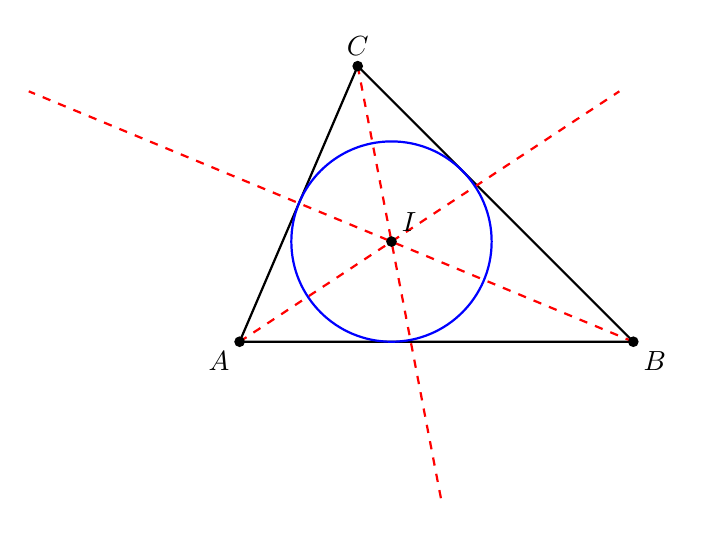
\begin{tikzpicture}[scale=1.0, thick]
  % 三角形 A=(0,0), B=(5,0), C=(1.5,3.5)
  \coordinate (A) at (0,0);
  \coordinate (B) at (5,0);
  \coordinate (C) at (1.5,3.5);
  \draw (A) -- (B) -- (C) -- cycle;
  % 计算内心：I = (a*A + b*B + c*C)/(a+b+c)
  % a = |BC|, b = |CA|, c = |AB|
  \pgfmathsetmacro{\ax}{1.5-5} \pgfmathsetmacro{\ay}{3.5}
  \pgfmathsetmacro{\aa}{sqrt(\ax*\ax+\ay*\ay)} % BC
  \pgfmathsetmacro{\bb}{sqrt(1.5*1.5+3.5*3.5)} % CA
  \pgfmathsetmacro{\cc}{5}                       % AB
  \pgfmathsetmacro{\sumw}{\aa+\bb+\cc}
  \pgfmathsetmacro{\Ix}{(\aa*0 + \bb*5 + \cc*1.5)/\sumw}
  \pgfmathsetmacro{\Iy}{(\aa*0 + \bb*0 + \cc*3.5)/\sumw}
  \coordinate (I) at (\Ix,\Iy);
  % 内切圆半径 = 面积/s; 面积=0.5*5*3.5=8.75; s=sumw/2
  \pgfmathsetmacro{\area}{0.5*5*3.5}
  \pgfmathsetmacro{\rr}{\area/(\sumw/2)}
  % 三条角平分线（延伸到对边）
  \draw[red, dashed] (A) -- ($(A)!1.0!(I)$) -- ($(A)!2.5!(I)$);
  \draw[red, dashed] (B) -- ($(B)!1.0!(I)$) -- ($(B)!2.5!(I)$);
  \draw[red, dashed] (C) -- ($(C)!1.0!(I)$) -- ($(C)!2.5!(I)$);
  % 内切圆
  \draw[blue] (I) circle (\rr);
  \filldraw (I) circle (1.5pt) node[above right] {$I$};
  \foreach \pt/\pos in {A/below left, B/below right, C/above} \filldraw (\pt) circle (1.5pt) node[\pos] {$\pt$};
\end{tikzpicture}
\end{document}
